\section{Taint-анализ}

Как уже было упомянуто, taint-анализ позволяет находить уязвимости в безопасности, отслеживая распространение непроверенных пользовательских данных по программе. Алгоритм действительно очень известный, ведь те или иные его модификации реализованы во многих популярных анализаторах. В частности, в некоторых из тех, что были рассмотрены во введении.

Одной из задач данной работы является реализация taint-анализа поверх символьной виртуальной машины UnitTestBot, что избавит описываемую технику от ложноположительных срабатываний. Таким образом, в результате модификации, единственным источником неточностей останется только само символьное исполнение.

\subsection{Конфигурация}

В процессе изучения темы не было найдено ни одного универсального формата конфигурации taint-анализа, а все известные мне статические анализаторы описывают свой собственный способ настройки. Таким образом, первая подзадача, которую нужно было решить ещё до модификации ядра символьной машины, "--- придумать схему конфигурации, где бы можно было описать правила (\verb|sources|, \verb|passes|, \verb|cleaners| и \verb|sinks|), с которыми будет вестись работа в дальнейшем. Формат должен быть удобен для пользователя, но в то же время предоставлять достаточно широкие возможности по настройке алгоритма. Исходя из перечисленных требований, в качестве базового языка разметки был взят YAML \cite{yaml}.

Теперь рассмотрим созданный формат в подробностях. Общая структура конфигурационного документа представлена ниже.

\begin{nocode}
sources:
  - <rule-1>
  - <rule-2>
  - < ... >
passes: [ ... ]
cleaners: [ ... ]
sinks: [ ... ]
\end{nocode}

То есть это просто списки правил, относящиеся к конкретному типу. Каждое правило имеет некоторый набор характеристик.

\begin{itemize}
    \item Уникальный идентификатор метода, которого описывает данное правило. Состоит из полного имени метода, включающего имя пакета и имя класса, а также из сигнатуры метода "--- набора типов его аргументов (ключ \verb|signature| в YAML).
    \item Некоторые условия \verb|conditions|, которые должны выполняться во время исполнения, чтобы правило сработало.
    \item Множество меток \verb|marks|, которыми оперирует правило.
    \item Набор конкретных действий по управлению метками, которые происходят при срабатывании правила (\verb|add-to|, \verb|get-from|, \verb|remove-from| или \verb|check| в зависимости от семантики правила).
\end{itemize}

Таким образом, одно правило, например \verb|taint source|, может выглядеть следующим образом.

\begin{nocode}
com.abc.ClassName.methodName:
  signature: [ <int>, _, <java.lang.Object> ]
  conditions:
    arg1: 
      not: [ -1, 1 ]
  add-to: [ this, arg2, return ]
  marks: user-input
\end{nocode}

Данное правило определяется для метода с именем \var{methodName} из класса \var{ClassName}, который находится в пакете \verb|com.abc|. Метод принимает ровно $3$ аргумента, первый из которых имеет тип \var{int}, второй может быть совершенно любым, а последний имеет тип \verb|java.lang.Object|. Ключ \var{signature} может быть не указан, тогда подходящей считается любая перегрузка \var{methodName}.

Срабатывание происходит только в том случае, когда первый аргумент (\var{arg1}) не равен ни $-1$, ни $1$ , что и указано по ключу \var{conditions} (список интерпретируется как логическое ИЛИ). Данный параметр является необязательным, в случае его отсутствия не будут проверены никакие условия. 

Описанный источник накладывает метку \verb|user-input| к переменным, соответствующим \var{this}, \var{arg2} и \var{return}. Другими словами, к объекту класса \var{ClassName}, на котором вызывается \var{methodName}, второму аргументу функции и возвращаемому значению. Причём по ключам \verb|add-to| и \var{marks} может лежать как список, так и одиночное значение "--- это сделано для удобства использования.

Остальные типы правил имеют такой же синтаксис, как и \verb|source|, за исключением ключа \verb|add-to|.

\begin{itemize}
    \item \verb|Taint pass| передаёт метки с одного множества объектов на другое, поэтому для него определяются два ключа: \verb|get-from| и \verb|add-to| соответственно. Причём на \verb|add-to| накладываются все указанные в \verb|marks| метки, если в \verb|get-from| есть хотя бы одна из них.
    \item \verb|Taint cleaner| удаляет метки с множества объектов, поэтому его ключ называется \verb|remove-from|.
    \item \verb|Taint sink| проверяет наличие некоторых меток в переменных, множество которых лежит по ключу \verb|check|.
\end{itemize}

Разработанный формат, с одной стороны, является лаконичным и читабельным для конечного пользователя, а с другой стороны, достаточно мощным для описания сложных правил или условий срабатывания.

Для описанной схемы конфигурации был реализован парсер, а также произведена необходимая интеграция с плагином для IntelliJ IDEA, чтобы программист мог настраивать taint-анализ под свой конкретный проект. 

Итоговый инструмент можно применять, и не составляя новых правил, для этого были добавлены распространённые источники и приёмники непроверенных данных. Приведём примеры для ясности. 

\begin{itemize}
    \item \verb|java.util.Scanner.nextLine| "--- это \verb|source|, накладывающий метку \verb|user-input| на возвращаемое значение.
    \item \verb|java.lang.String.concat| "--- это \verb|pass|, который добавляет к возвращаемому значению все метки, полученные из \verb|this| и \verb|arg1|.
    \item \verb|java.lang.String.isEmpty| "--- это \verb|cleaner|, который удаляет все метки из объекта \verb|this| в том случае, если \verb|return| равняется \verb|true| (пустая строка не может содержать вредоносных данных).
    \item \verb|java.sql.Statement.execute| "--- это \verb|sink| для меток \verb|user-input|.
\end{itemize}

\subsection{Детали реализации}

В данном подразделе будут описаны общие концепции интеграции taint-анализа и символьного исполнения, а также детали реализации в UnitTestBot.

\subsubsection{Общие концепции}

Ключевая идея состоит в том, чтобы для каждой символьной переменной поддерживать набор меток, наложенных на неё в процессе работы символьной машины (подробнее о символьном исполнении описано в разделе \ref{sec-sym-exec}). Эти наборы могут изменяться только при вызове метода, для которого существует правило в конфигурации (\verb|source|, \verb|pass|, \verb|cleaner| или \verb|sink|). 

Общий вид обработки источника представлен в алгоритме \ref{source-algo}. Для каждого заданного в конфигурации правила \verb|rule|, которое относится к текущему методу, и для каждой сущности \verb|entity| внутри него (\verb|this|, \verb|return| или аргумент метода) алгоритм получает соответствующую ему символьную переменную \verb|symbol|, после чего добавляет к её набору меток \verb|marks[symbol]| метки из \verb|rule|.

\begin{algorithm}[hbt!]
\caption{Обработка источника помеченных данных}\label{source-algo}

\SetKwProg{ProcessTaintSource}{ProcessTaintSource}{}{}
\ProcessTaintSource{$(config, stmt)$}{
    \KwData{$config$ "--- набор правил taint-анализа}
    \KwData{$stmt$ "--- текущая инструкция (вызов метода)}
    
    $rules = config.getSourcesBy(stmt)$\;
    \ForEach{$rule \in rules$}{
        \ForEach{$entity \in rule.entities$}{
            $symbol \gets getSymbolicValue(stmt, entity)$\;
            $marks[symbol] = marks[symbol] \cup rule.marks$\;
        }
    }
}
\end{algorithm}

Алгоритм обработки правил \verb|taint sink| (\ref{sink-algo}) выглядит также, с той лишь разницей, что вместо добавления символьная машина проверяет наличие запрещённых меток \verb|rule.marks| во множестве \verb|marks[symbol]|, и, если пересечение множеств не пусто, то сообщает о найденной уязвимости.

\begin{algorithm}[hbt!]
\caption{Обработка приёмника помеченных данных}\label{sink-algo}

\SetKwProg{ProcessTaintSink}{ProcessTaintSink}{}{}
\ProcessTaintSink{$(config, stmt)$}{
    \KwData{$config$ "--- набор правил taint-анализа}
    \KwData{$stmt$ "--- текущая инструкция (вызов метода)}
    
    $rules = config.getSinksBy(stmt)$\;
    \ForEach{$rule \in rules$}{
        \ForEach{$entity \in rule.entities$}{
            $symbol \gets getSymbolicValue(stmt, entity)$\;
            \If{$marks[symbol] \cap rule.marks \neq \varnothing $}{
                $reportProblem()$\;
            }
        }
    }
}
\end{algorithm}

Алгоритмы для правил \verb|taint pass| и \verb|cleaner| аналогичны представленным выше, за исключением строки с изменением \verb|marks| (в соответствии со своей семантикой), поэтому для краткости в тексте работы не приводятся.

\subsubsection{Модификация символьной машины}

Теперь подробно рассмотрим детали встраивания taint-анализа в выбранную символьную виртуальную машину.

Общий вид работы UnitTestBot выглядит следующим образом. На вход инструменту поступает программа в виде инструкций байт-кода. Объект \verb|PathSelector| определяет порядок обхода символьных состояний, \verb|Traverser| отвечает за обработку одной инструкции, а также поддерживает символьную память \verb|Memory| и систему типов \verb|TypeRegistry| в актуальном виде. В терминальном состоянии делается запрос к SMT-решателю с целью определить выполнимость пройденного пути и найти для него конкретные входные данные. Более подробное описание ключевых мест в процессе работы UnitTestBot представлены в разделе \ref{sec-utbot-arch}.

Основная идея реализованного подхода состоит в том, что каждой символьной переменной сопоставляется \verb|taint vector| "--- 64-битное значение, каждый бит \var{i} которого отвечает за наличие метки с номером \var{i} в этом объекте. После чего, в процессе работы символьной машины, эти сопоставления поддерживаются и обновляются в соответствии с классическим алгоритмом taint-анализа.

Сделанные в данной работе изменения в большинстве своём затрагивают классы \verb|Traverser| и \verb|Memory|. Также, были добавлены новые компоненты \verb|TaintModel|, \verb|TaintMarkRegistry| и \verb|TaintMarkManager|. На рис. \ref{taint-arch} представлена высокоуровневая диаграмма разработанного модуля. Разберём зону ответственности каждой сущности подробнее.

\begin{figure}[ht]
    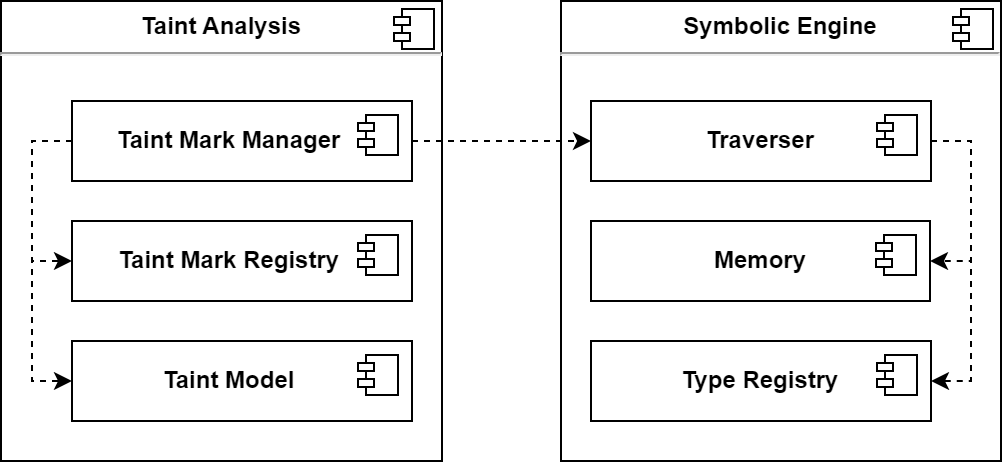
\includegraphics[scale=0.35]{images/taint-arch-tr-200.png}
    \centering\caption{\label{taint-arch} Архитектура модуля Taint-анализа.}
\end{figure}

Объект класса \verb|TaintMarkRegistry| хранит сопоставление между именем метки и её порядковым номером от $0$ до $63$. Видим, что количество меток, которые могут быть одновременно задействованы в анализе, ограничено числом $64$. Однако, во-первых, этого хватает для почти любого разумного примера, а во-вторых, решение было обусловлено вопросами производительности "--- операции с типом данных \verb|Long| совершаются намного быстрее, чем если бы был использован битовый массив произвольного размера. 

Компонент \verb|TaintModel| отвечает за предоставление доступа к конфигурации. В частности, он определяет способ преобразования условий (значение по ключу \verb|conditions| в YAML-документе) в логические выражения над символьными переменными. Отметим, что сам \verb|TaintModel| не выполняет никаких действий, а лишь предоставляет процедуру, которую можно запустить, уже имея на руках \verb|Memory| и \verb|TypeRegistry|.

\verb|Memory| занимается хранением значений \verb|taint vector| для символьных переменных. В этом же классе были реализованы простые функции для обновления векторов и их получения по адресу символьного объекта. Вся сложная логика по добавлению и удалению меток, опирающаяся на теорию taint-анализа, была написана в отдельной сущности \verb|TaintMarkManager|. Другими словами, этот класс оборачивает низкоуровневую работу с памятью в понятные с точки зрения предметной области операции.

Обновление информации о помеченных переменных происходит в процессе работы \verb|Traverser|. Перед каждой из \verb|invoke| инструкций, которые соответствуют запуску некоторого метода в пользовательском коде, вызывается специальный обработчик \verb|processTaintSink|, а уже после инструкции \verb|invoke| вызываются обработчики \verb|processTaintSource|, \verb|processTaintPass| и \verb|processTaintCleaner|. Такой порядок связан с тем, что всем правилам, кроме приёмников, нужен результат работы функции. При этом факт передачи заражённых данных происходит в момент запуска функции-приёмника, поэтому сообщить о найденной уязвимости можно ещё до её выполнения. 

Перечисленные обработчики правил обращаются к \verb|TaintModel|, чтобы проверить, есть ли информация про рассматриваемый метод в конфигурации, и, если есть, то получить её. Функция \verb|processTaintSink| запрашивает у \verb|TaintMarkManager| данные об уже выставленных метках и добавляет ограничения в SMT-решатель, выполнение которых соответствует обнаружению дефекта. Остальные обработчики изменяют символьную память \verb|Memory| через тот же \verb|TaintMarkManager|, добавляя и удаляя метки у выбранных символьных объектов.

В результате удаётся не только обнаружить возможные уязвимости, но и сгенерировать конкретные входные данные, запуск программы на которых покажет, по какому маршруту заражённые переменные могут проникнуть в критические секции кода.

\subsubsection{Модификация генератора кода}

Результатом работы UnitTestBot, помимо добавленного в данной работе отчёта SARIF, являются тесты. Другими словами, на каждом найденном тестовом случае запускается \verb|CodeGenerator|, который должен оформить тест в виде кода на языке Java. Причём, если тест ведёт к выбрасыванию необработанного исключения, то он не должен проходить.

Ошибки, которые получаются в результате работы модуля taint-анализа, не являются настоящими с точки зрения языка, так как это не исключения. Однако хотелось бы всё равно выделить такие тесты как провальные, поэтому генератор кода был изменён таким образом, чтобы в конце каждого теста добавлялась искусственная ошибка, которая бы и обеспечивала падение.

\begin{code}
Assertions.fail(
    "'java.lang.String' marked 'user-input'
     was passed into 'Statement.execute' method"
);
\end{code}

Предоставленное решение оказалось очень удачным, ведь оно позволило автоматически получить интеграцию с отчётами SARIF и визуализацией результатов во вкладке \verb|Problems view| в IntelliJ IDEA. Найденный тестовый случай теперь трактуется как настоящее исключение, а для них уже написана вся нужная логика.

\subsection{Пример работы}

Рассмотрим пример работы реализованного модуля на классе \verb|User|. 

\begin{code}
public class User {

    String getLogin() { /* some logic */ }

    String getPassword() { /* some logic */ }

    String userInfo(String login, String password) {
        return login + "#" + password;
    }

    void printUserInfo() {
        var login = getLogin();
        var password = getPassword();
        var info = userInfo(login, password);
        System.out.println(info);
    }
}
\end{code}

Метод \verb|getPassword| возвращает чувствительные данные, которые ни в коем случае не должны утечь из приложения, а программист печатает их в стандартный поток вывода, что является серьёзной ошибкой.

Сначала напишем конфигурацию, которая выражает сказанную мысль, и сохраним её в файл \verb|./.idea/utbot-taint-config.yaml|, откуда её сможет прочесть анализатор.

\begin{nocode}
sources:
  - User.getPassword:
      add-to: return
      marks: sensitive-data
passes:
  - User.getUserInfo:
      get-from: [ arg1, arg2 ]
      add-to: return
      marks: [] # all
sinks:
  - java.io.PrintStream.println:
      check: arg1
      marks: sensitive-data
\end{nocode}

Теперь запускаем UnitTestBot с помощью плагина для IntelliJ IDEA и смотрим на полученный результат.

Во-первых, сгенерировался тест, по которому понятно, что модуль taint-анализа нашёл уязвимость.

\begin{code}
@Test
public void testPrintUserInfo1() {
    User user = new User();
    user.printUserInfo();
    fail(
        "'java.lang.String' marked 'sensitive-data' 
         was passed into 'PrintStream.println' method"
    );
}
\end{code}

Во-вторых, появилась панель \verb|Problems view| (рис. \ref{problems-view-taint}), где отображена найденная проблема в виде результата статического анализа.

Разберём чуть подробнее внутренности работы модуля на данном примере.

После выполнения метода \verb|getPassword| символ, соответствующий переменной \verb|password|, помечается как \verb|sensitite-data| (возводится нулевой бит в его \verb|taint vector|).

После вызова \verb|userInfo| помечается также переменная \verb|info|, так как \verb|userInfo| "--- это \verb|taint pass|, который добавляет к возвращаемому значению все метки, собранные из обоих своих аргументов.

Перед печатью \verb|info| на консоль, функция-обработчик \verb|processTaintSink| добавляет ограничение в SMT-решатель, выполнение которого соответствует выбрасыванию нашего фиктивного исключения. Логическая формула для данного пути оказывается выполнима, поэтому анализатор сообщает о найденной ошибке, что мы в итоге и наблюдаем.
